\documentclass{beamer}
\usetheme{AnnArbor}

\title{Corporate default prediction}
\subtitle{Statistics for Data science - AEM University of Brescia}
\author{Mateusz Dadej}
\date{\today}

\begin{document}

\begin{frame}
\titlepage
\end{frame}

\begin{frame}{Research questions}
\begin{itemize}
\item What are the consequences of applying different resampling methods? Is the more complex the better?
\item What's the most efficient way to make a model of a corporate probability of default?
\end{itemize}
\end{frame}

\begin{frame}{Overview of data: Basic information}

\begin{itemize}
\item Data is sourced from Orbis - Database with private companies
\item Geographical location of companies are developed countries in Europe 
\item observations were filtered with following criteria:
	\begin{itemize}
	\item Active, bancrupt or dissolved at time $t$
	\item With known value of some financial ratios at time $t-1$
	\item Standardised legal form: Private and public limited company
	\item Entity type: corporate
	\item Higher than 5 number of employees at time $t-1$
	\end{itemize}

\end{itemize}

\end{frame}

\begin{frame}{Overview of data}
\begin{center}
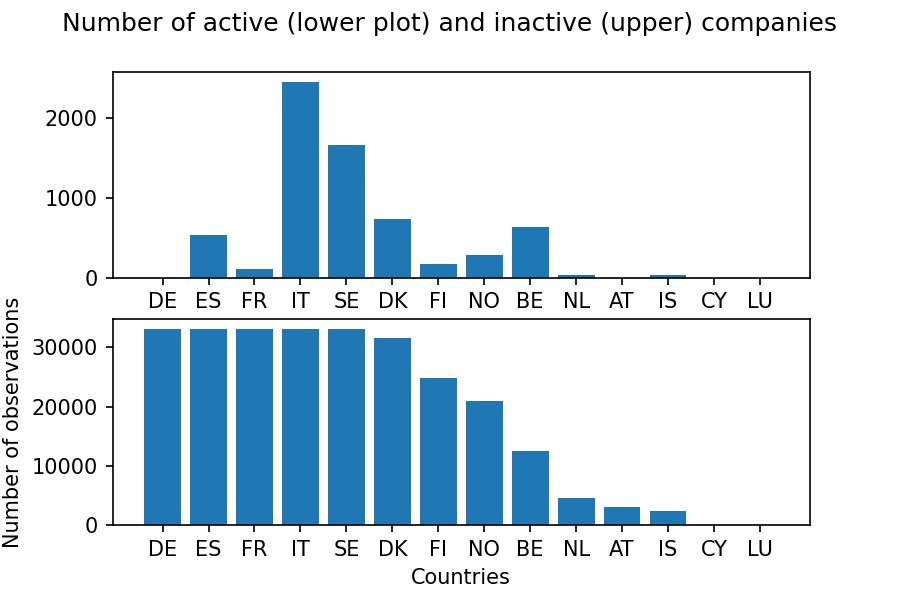
\includegraphics[scale=0.7]{img/country_n.png}
\end{center}
\end{frame}

\begin{frame}{Data preprocessing}

\begin{itemize}
\item Variables with more than $25$\% not available values were dropped
\item Categorical variables were one-hot-encoded
\item NAs were imputed with the median of a given variable
\item Preprocessed dataset was split into training (80\%) and testing dataset 

\end{itemize}

\

For feature engineering, additional 20 new variables were introduced from initial 30, briefly:

\begin{itemize}
\item For some financial data like revenue, net proft, a relative change from previous year was introduced
\item Most of the original variables were a standard positions from finacial statement, thus financial ratios were introduced with some basic arithmetic operations.

\end{itemize} 

\end{frame}

\begin{frame}{Resampling methods}
Corporate default data is known to have a huge class imbalance problem. 

\

In order to adress the problem and investigate their modeling consequences, I further apply 3 resampling methods to the training dataset:

\begin{itemize}
\item Oversampling
\item Undersampling
\item Synthetic Minority Over-sampling Technique (SMOTE) [N. Chawla, et. al, 2002] + Undersampling 
\end{itemize}

\

Further modeling workflow is done for datasets resampled with each of the methods above, in order to compere them.
\end{frame}

\begin{frame}{Resampling methods - SMOTE}
\begin{itemize}
\item Model-based oversampling technique
\item synthetic observations - sampled from the feature space around N-nearest neighbours (5 neighbours in this project). 
\item The only method used that introduces some randomness
\item combined with undersampling, as the original paper suggests [N. Chawla, et. al, 2002]
\end{itemize}
\end{frame}

\begin{frame}{Resampling methods}
\begin{center}
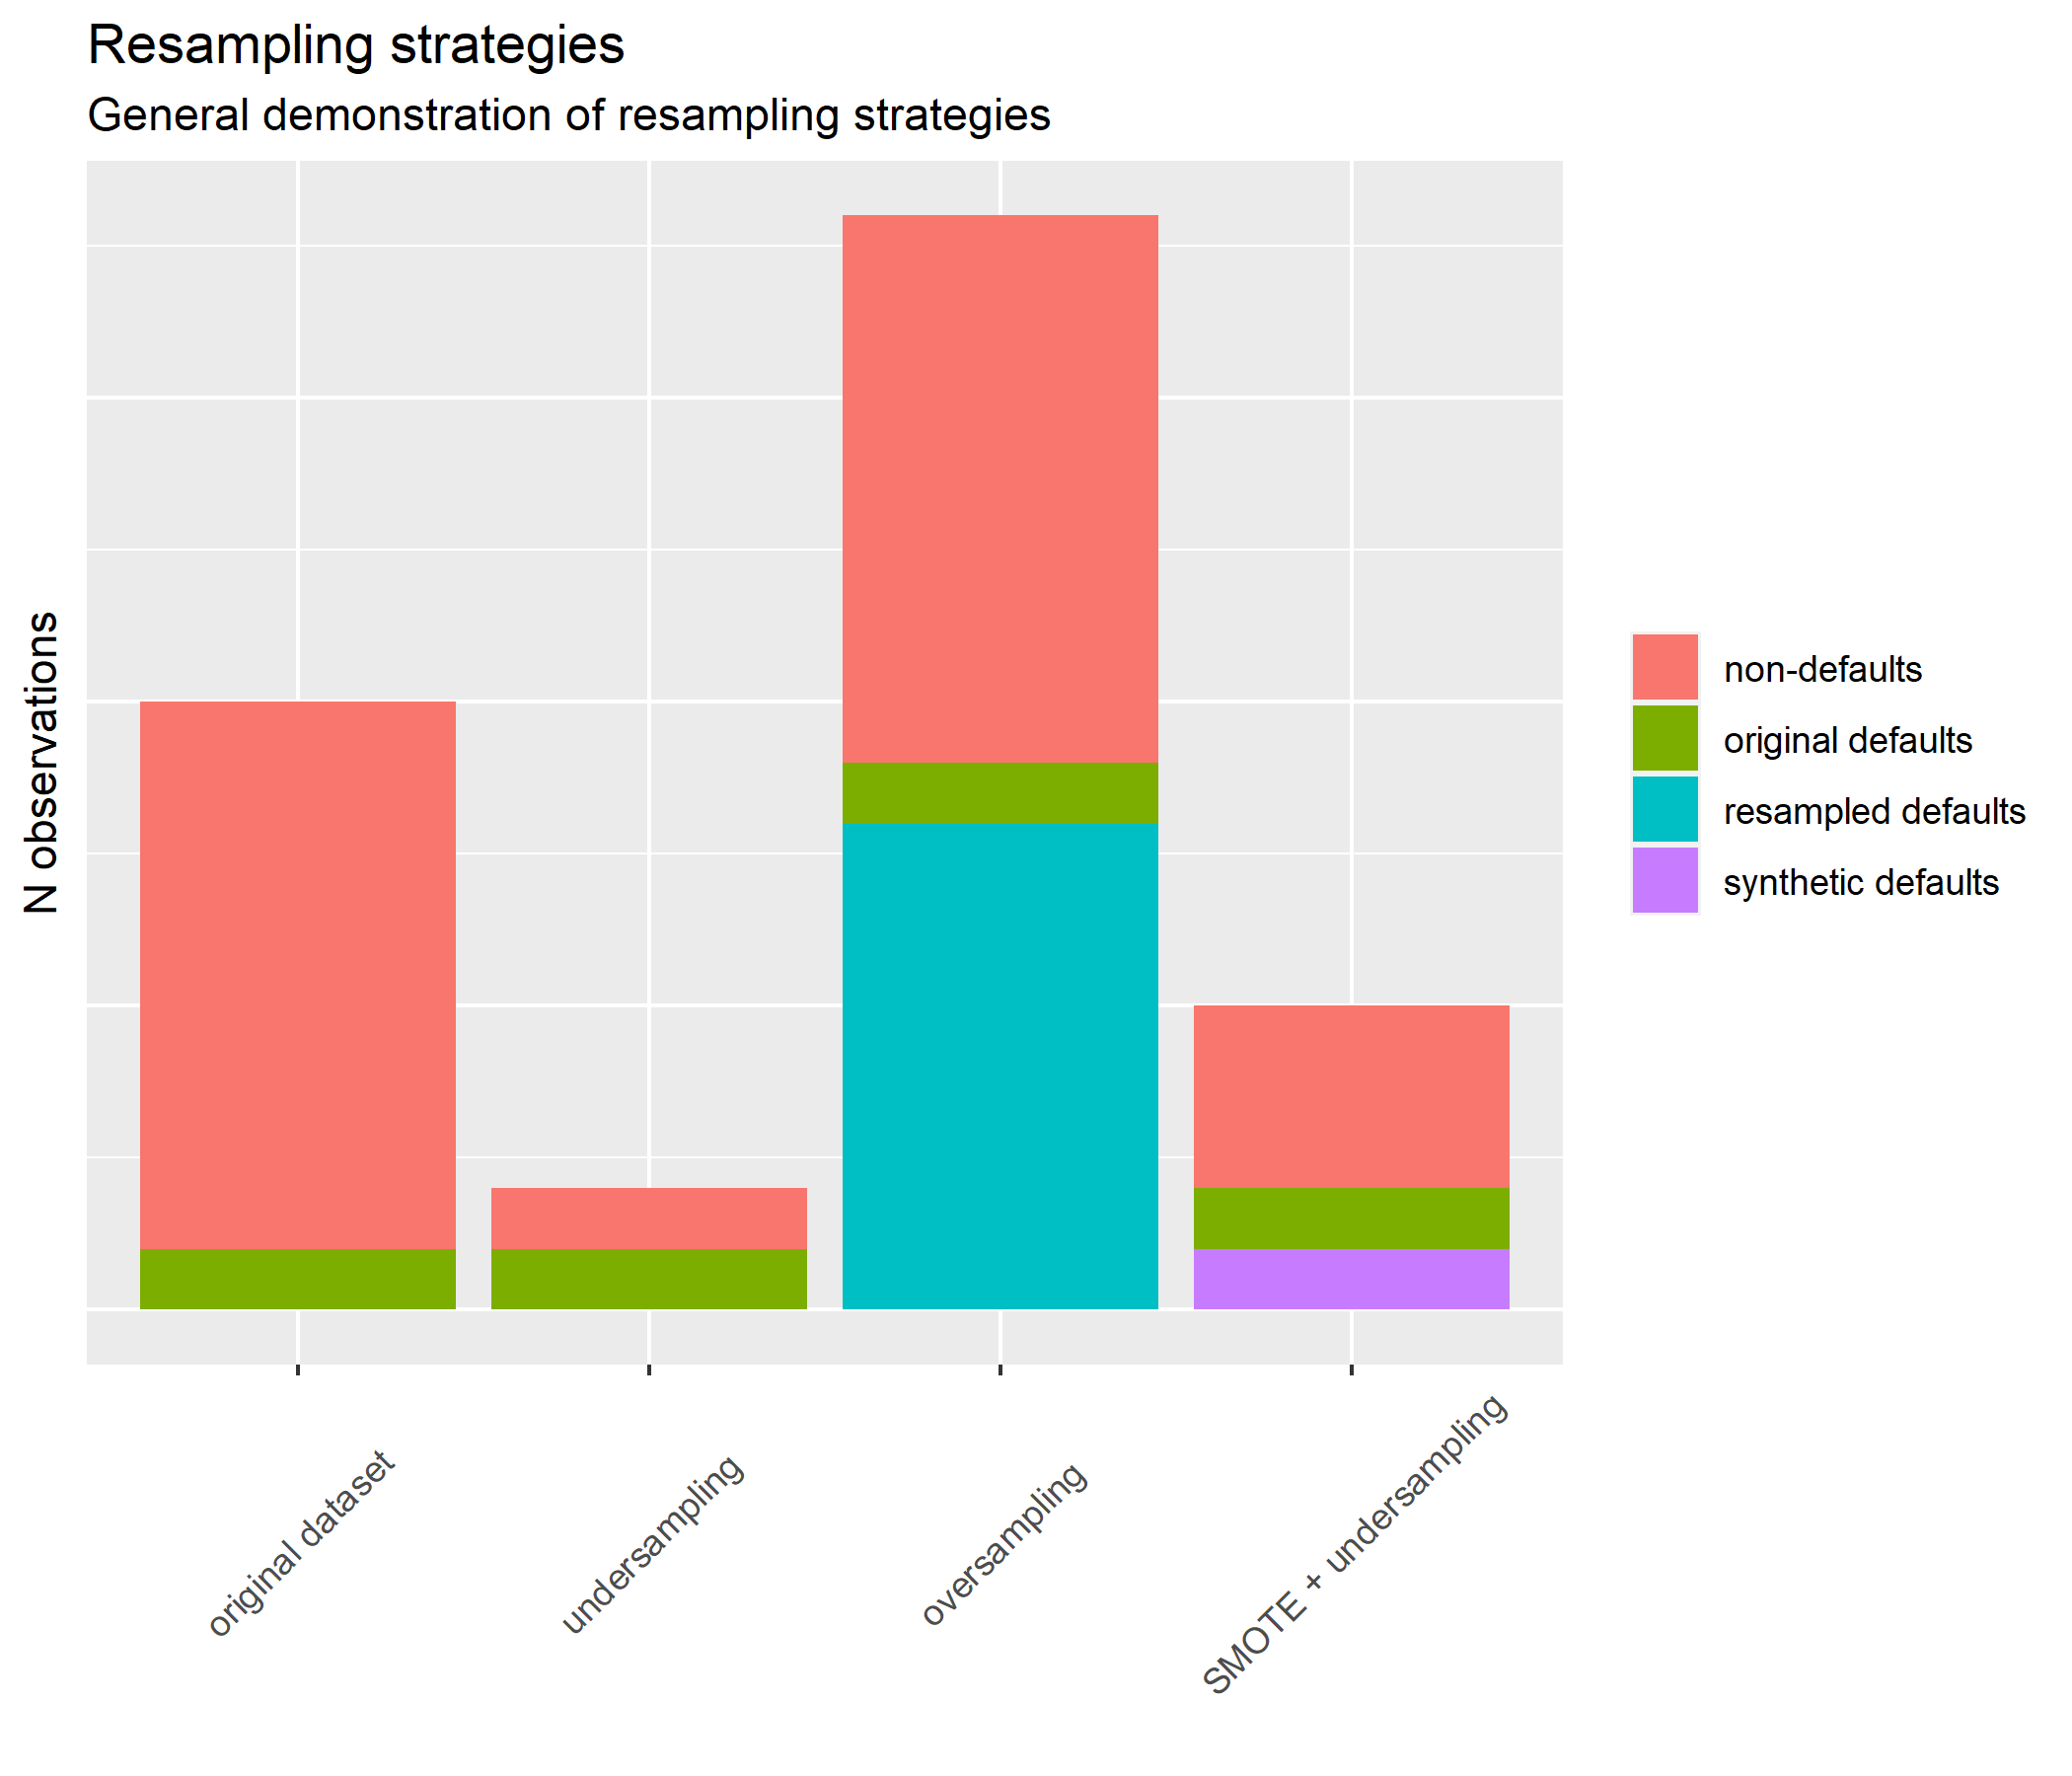
\includegraphics[scale=0.5]{img/resampling_strat.png}
\end{center}
\end{frame}

\begin{frame}{Resampling methods - stratified resampling}

\begin{itemize}
\item Problem: Imbalance not only on the dataset level but also between countries (see: slide 4)
\item Consequence: ML favor countries with imbalance e.g:

\begin{itemize}
	\item IT with highest number of defaults $\rightarrow$ ML gives higher PD to Italian corporates
	\item Is it economically sensible? (no, mostly sampling error)
	\item Opposite effect for France
\end{itemize}

\item Solution: weighted (undersampling) oversampling with weights (negatively) proportional to the share of defaults in the original dataset
\item Effect: The trainning datasets have effectively balanced classes between countries
\end{itemize}
\end{frame}


\begin{frame}{Applied models (1/3): Penalized logistic regression}

$$\min_{w,c} \frac{1-\rho}{2} \beta^{T}\beta + \rho ||\beta||_1 + C \sum_{i-1}^n \ln e^{-y_i(X_i^T \beta + c)}+1$$

Where:

\begin{itemize}
\item $\rho$ parameter regulating preference for l-2 or l-1 regularizaton
\item C paraemters regulating preference to regularization
\end{itemize}

\

Both of the parameters above were tuned with a grid search over corss validated results.


\end{frame}

\begin{frame}{Applied models (2/3): XGBoost - Gradient boosted decision trees}

\begin{itemize}
\item A workhorse ML model, based on an ensemble of decision trees [T. Chen, C. Guestrin, 2016].
\item Trained with a gradient boosting algorithm based on Friedman et al. 2000
\item The model is trained in a sequential way, each training round consists of function estimated from previous round and a newly trained one.
\item The objective function both tries to minimize log-loss and a regularization term, which penalizes number of leaves and a l-2 norm of leaf score
\item all in all, a complex model....

\item In herein project, the hyperparameters were tuned with random search.

\end{itemize}

\end{frame}

\begin{frame}{Applied models (3/3): Multilayer perceptron}

\begin{itemize}
\item Basic "vanilla" model of artificial neural networks
\item Estimates weights of "neurons" iteratively with backpropagation
\item Just like the previous model, can generalize non-linear patterns and has a regularization in a objective function
\end{itemize}

\

For this project, the hyperparameters were tuned with a random search.

\end{frame}

\begin{frame}{model fitness comparison - ROC}

\begin{center}
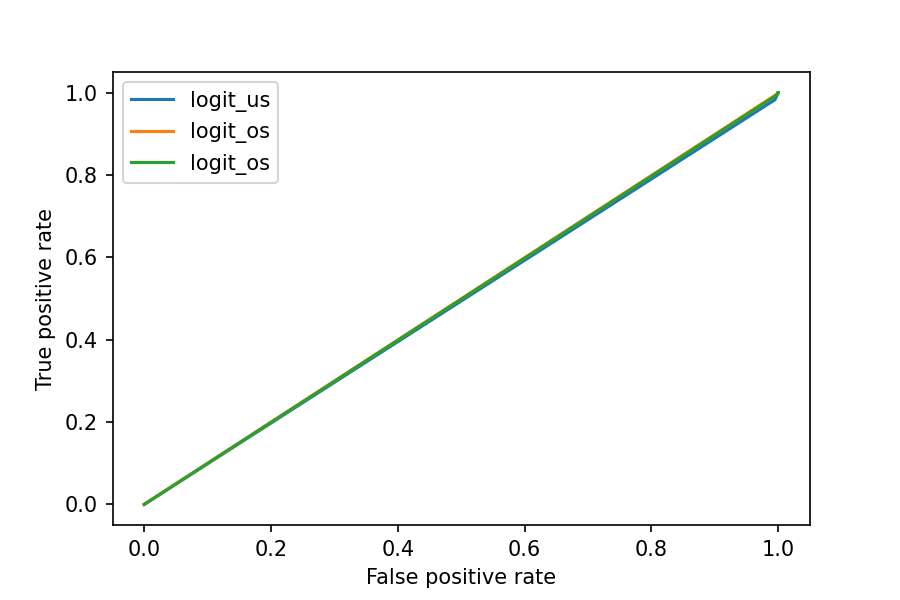
\includegraphics[scale=0.5]{img/log_roc.png}
\end{center}

\begin{itemize}
\item Fairly well fit to the data, a weaker one with SMOTE
\item SMOTE indtroduced some jumps with respect to the change of the threshold
\end{itemize}

\end{frame}

\begin{frame}{model fitness comparison - ROC}

\begin{center}
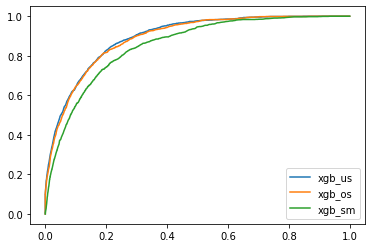
\includegraphics[scale=0.54]{img/xgb_roc.png}
\end{center}

\begin{itemize}
\item Similar shape
\item Surprisingly, SMOTE laggs behind other methods
\end{itemize}

\end{frame}

\begin{frame}{model fitness comparison - ROC}

\begin{center}
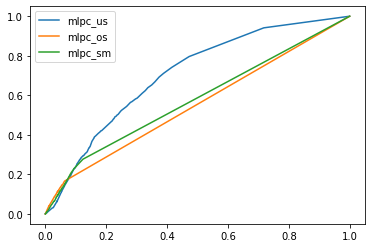
\includegraphics[scale=0.55]{img/mlpc_roc.png}
\end{center}

\begin{itemize}
\item Different shape for every method
\item Once again, the SMOTE method is worse than the rest
\end{itemize}

\end{frame}

\begin{frame}{TPR, TNR vs. threshold}
\begin{columns} 
% Column 1
\fontsize{9pt}{7.2}\selectfont

    \begin{column}{.5\textwidth}
    \begin{center}
        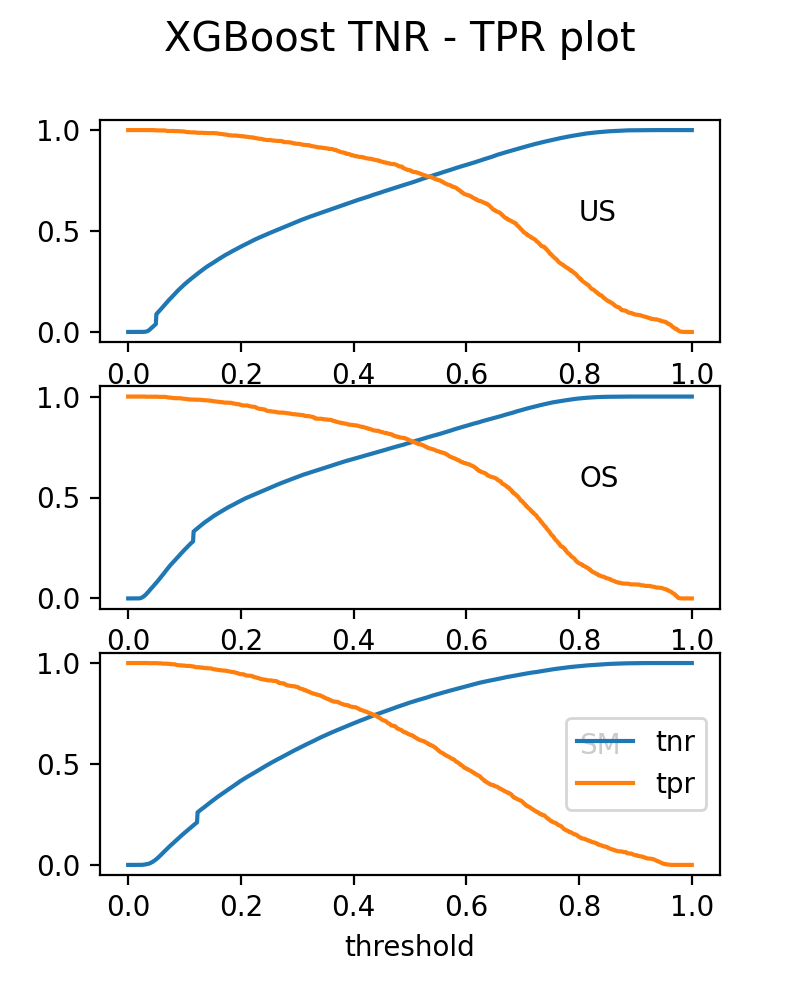
\includegraphics[scale=0.55]{img/xgb_tnr_tpr.png}
		\end{center}
    \end{column}
% Column 2    
    \begin{column}{.5\textwidth}
        \begin{center}
        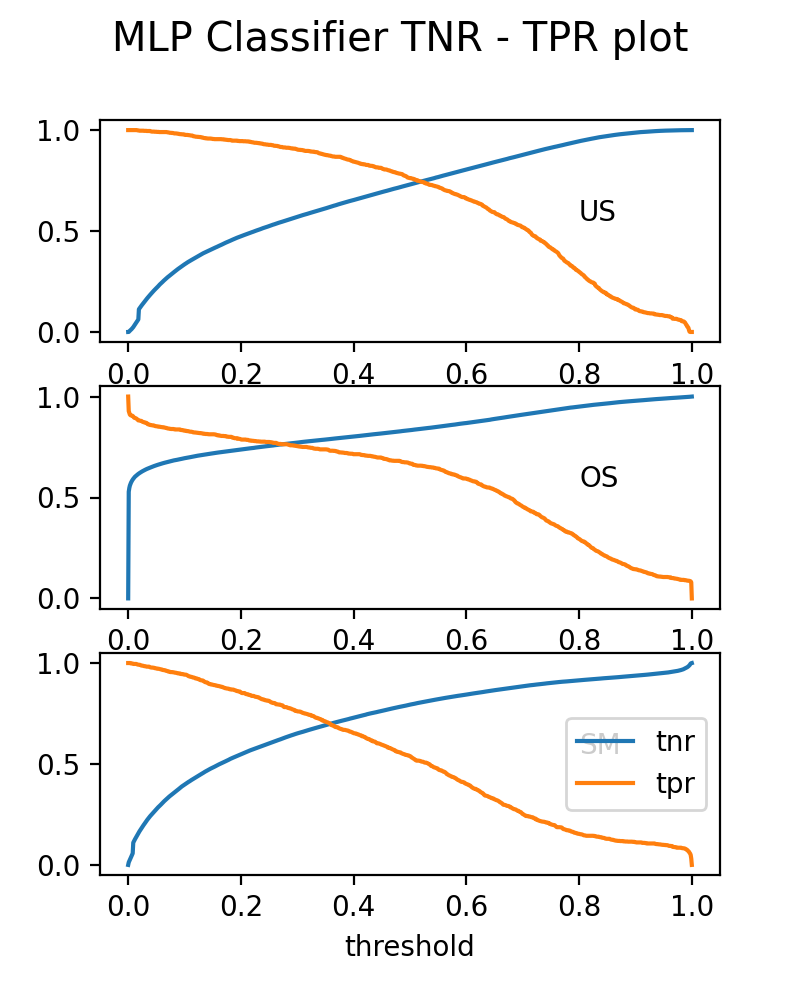
\includegraphics[scale=0.55]{img/mlpc_tnr_tpr.png}
		\end{center}
    \end{column}%
    
\end{columns}

\end{frame}

\begin{frame}{Metrics with optimal thresholds}

\begin{itemize}
\item Optimal threshold w.r.t balanced accuracy
\item note, it's in-sample opimtal (best case scenario)
\end{itemize}

\begin{center}
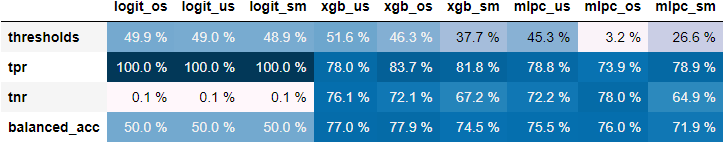
\includegraphics[scale=0.6]{img/max_balance_table.png}
\end{center}
\end{frame}

\begin{frame}{Base case metrics comparison}

\begin{itemize}
\item Metrics calculated with $50$\% threshold (base case)
\end{itemize}

\begin{center}
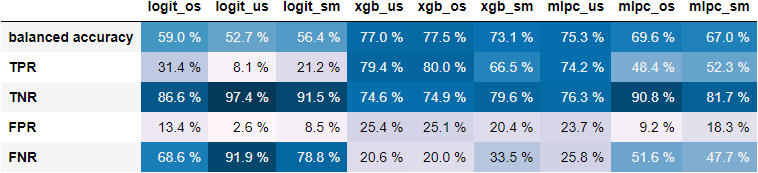
\includegraphics[scale=0.6]{img/balance_acc_table.png}
\end{center}
\end{frame}

\begin{frame}{Feature importance}

\begin{itemize}
\item Surprisingly high importance of variables in absolute values
\item Smaller country effect than before stratified resampling
\item Different patternrecognition between ML models (MLPC - sectors, XGB - ratios)
\end{itemize}
\begin{columns} 
% Column 1
\fontsize{9pt}{7.2}\selectfont

    \begin{column}{.5\textwidth}
    \begin{center}
        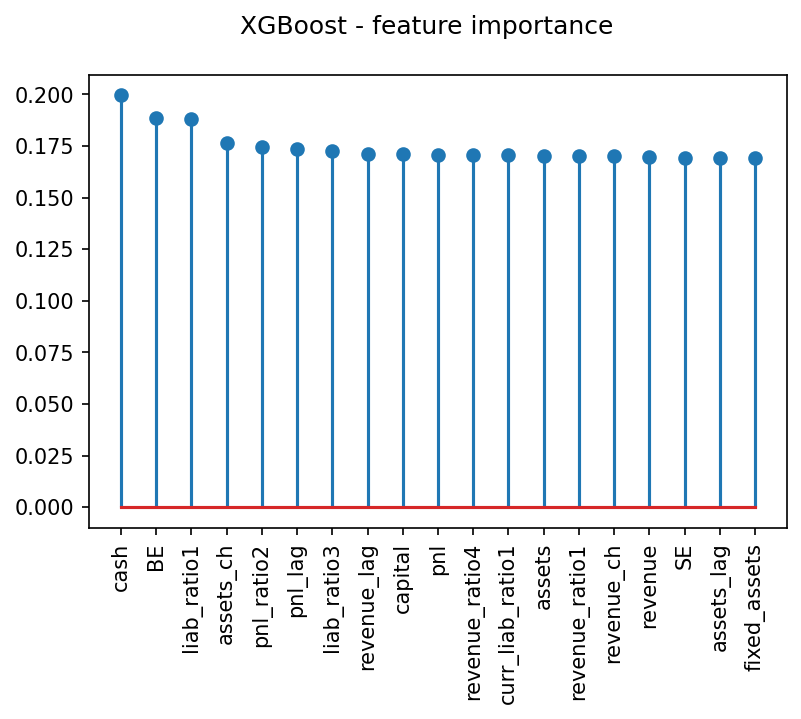
\includegraphics[scale=0.42]{img/xgb_exp.png}
		\end{center}
    \end{column}
% Column 2    
    \begin{column}{.5\textwidth}
        \begin{center}
        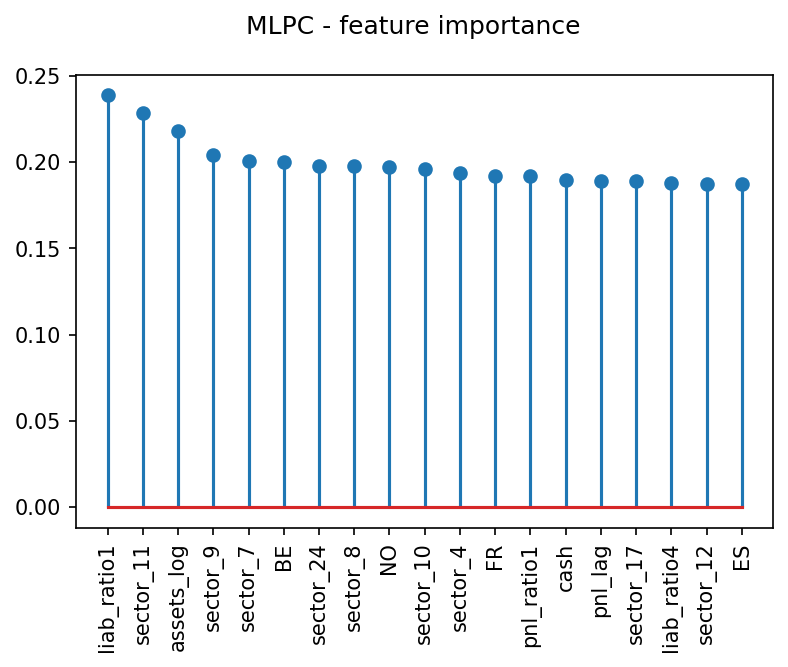
\includegraphics[scale=0.42]{img/mlpc_exp.png}
		\end{center}
    \end{column}%
    
\end{columns}
\end{frame}

\begin{frame}{Feature importance without stratified resampling}

\begin{center}
        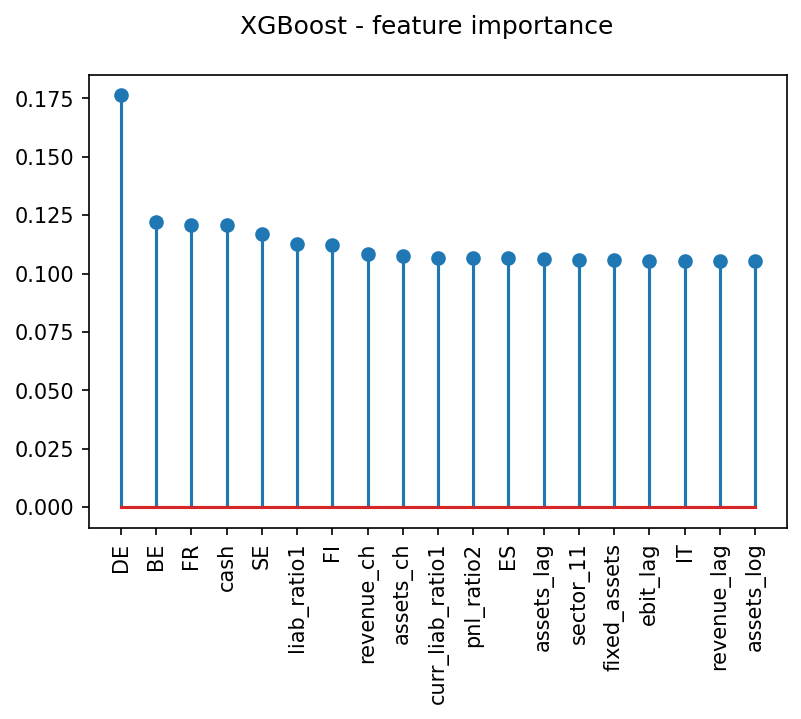
\includegraphics[scale=0.42]{img/no_country_effect/xgb_exp.png}
\end{center}

\begin{center}
        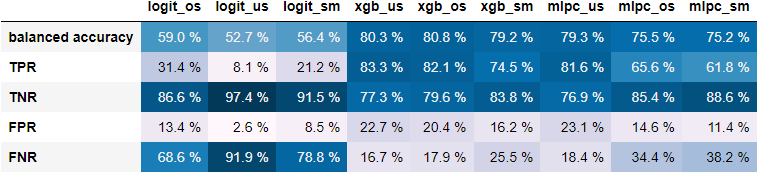
\includegraphics[scale=0.35]{img/no_country_effect/balance_acc_table.png}
\end{center}

\end{frame}

\begin{frame}{Case study: Energia Siciliana S.R.L}

\begin{itemize}
\item Big contribution to the variables in absolute levels
\item correctly predicted bankcruptcy 1 year before (76,6\%)
\end{itemize}


\begin{center}
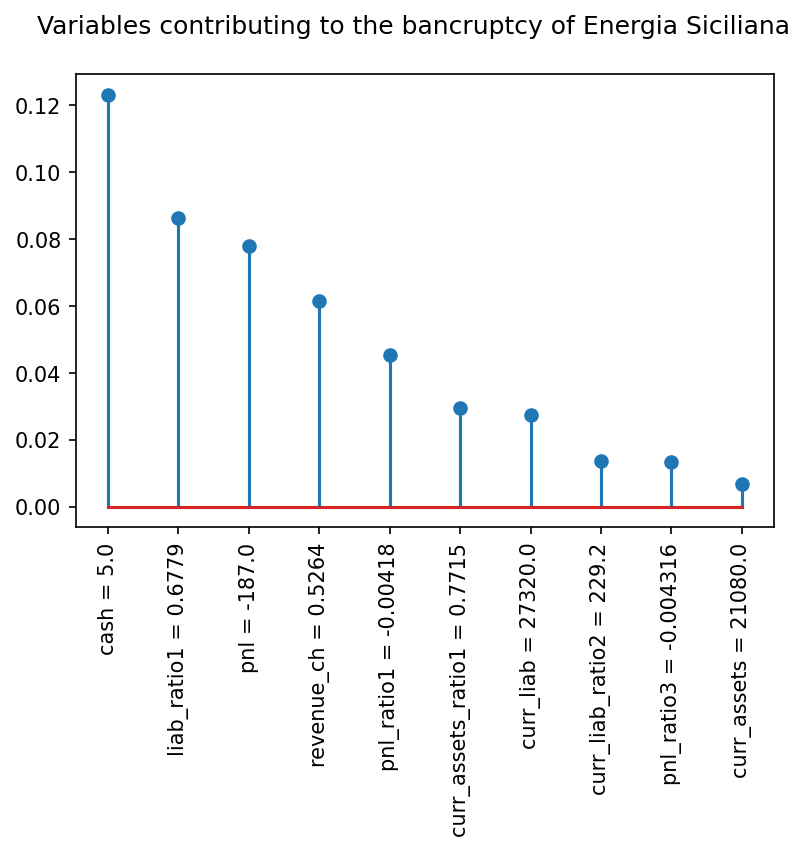
\includegraphics[scale=0.4]{img/energia_plot.png}
\end{center}
\end{frame}

\begin{frame}{further research}
\begin{itemize}
\item What's the value-added of having single model for each country vs. a single model to rule them all?

\item Choose final model:

\begin{itemize}
\item best combination of resampling technique and algorithm
\item perhaps average few models
\item spend more time optimizing single model
\item What are the best metrics we can get?
\end{itemize}

\item simulating a credit portfolio for a given empirical parameters (RR, ROI, default rate) Is the model profitable?
\end{itemize}
\end{frame}

\begin{frame}{References}

\begin{itemize}
\item N. V. Chawla, et. al, SMOTE: Synthetic Minority Over-sampling Technique, Journal of Artificial Intelligence Research 16, 2002
\item T. Chen, C. Guestrin, XGBoost: A Scalable Tree Boosting System, 2016
\item J. Friedman, T. Hastie, and R. Tibshirani. Additive logistic
regression: a statistical view of boosting. Annals of
Statistics
\end{itemize}
\end{frame}
\end{document}



